
    \chapter{Implementação e Evolução Técnica}

    \section{Tecnologias e Metodologias Utilizadas}
    O \textbf{OmniAI SDK} foi desenvolvido em Kotlin Multiplatform \cite{kmp_ref} com \textit{targets} JVM e JavaScript/Node.js.
    A escolha de KMP permite partilhar o domínio, os contratos, as portas, os \textit{adapters} principais e parte da lógica geral entre plataformas, mantendo implementações específicas quando o ambiente o exige \cite{kotlin_multiplatform}. A serialização dos contratos é baseada em Kotlinx Serialization\cite{serialization_ref}, o que facilita a definição explícita dos modelos JSON que foram apresentados anteriormente.

    O \textit{core} do \textbf{OmniAI SDK} é estritamente agnóstico em relação a \textit{frameworks} web e mecanismos de transporte HTTP. Contudo, para fornecer uma solução imediatamente utilizável, o projeto inclui módulos de integração baseados na \textit{framework} Ktor\cite{ktor_ref}. Estes módulos opcionais oferecem implementações de referência tanto para a execução de pedidos aos fornecedores (\textit{client-side}) como para a exposição das rotas da \textbf{Gateway} (\textit{server-side}). A \textbf{OmniAI Gateway} instanciada como Prova de Conceito (PoC) tira partido destas implementações prontas a usar. No entanto, a adoção do \textbf{OmniAI SDK} não obriga ao uso do Ktor, a arquitetura garante que qualquer utilizador possa descartar estes módulos e implementar os adaptadores de rede utilizando a tecnologia da sua preferência, como o Spring\cite{ref_spring} por exemplo, entre outros.

    As ferramentas de desenvolvimento incluíram Git, IntelliJ IDEA, o cliente \textbf{HTTP} do IDE para pedidos \textbf{REST}, \textbf{Docker Compose} para \textbf{Logto} \cite{logto_docs}, \textbf{PostgreSQL} \cite{postgresql_ref}, \textbf{OpenTelemetry Collector} \cite{opentelemetry_what_is}, \textbf{Prometheus} \cite{prometheus_ref} e \textbf{Grafana} \cite{grafana_ref}, além de clientes reais como \textbf{Claude Code} e SDKs oficiais dos fornecedores. Também foram usados assistentes de apoio, como Gemini no \textit{browser} e agentes de programação como o \textbf{Antigravity} e \textbf{Codex}, para pesquisa, comparação de documentação e aceleração de tarefas, mantendo a validação no código, nos testes e nos cenários executados. Foi criada uma \textit{pipeline} de \textbf{Continuous Integration} (CI) \cite{CI_ref}  que executa \texttt{./gradlew clean build}  e \texttt{./gradlew check}, que realizam build ao projeto e executam testes unitarios, como passo evolutivo, está prevista a criação de uma \textit{pipeline} de \textbf{Continuous Deployment} (CD) para publicar as versões do nosso \textit{Software Development Kit},o \textbf{OmniAI SDK} em Maven e NPM.

    \section{A Primeira Iteração da \textit{Gateway}}

    A primeira iteração do projeto consistiu numa \textbf{Gateway} \textbf{HTTP} construída diretamente, responsável por receber pedidos de clientes e encaminhá-los para fornecedores de inferência. Esta fase foi útil para validar rapidamente a viabilidade da solução, testar pedidos reais e compreender diferenças práticas entre as diferentes API's dos fornecedores, neste caso da \textbf{OpenAI} \cite{openai_api}, \textbf{Anthropic}\cite{anthropic_api} e \textbf{Gemini}\cite{google_gemini_api}.

    À medida que o sistema cresceu, essa abordagem revelou acoplamento excessivo. A tradução entre contratos, a configuração dos fornecedores, a autenticação, o tratamento de erros e o encaminhamento de pedidos começaram a concentrar-se na própria aplicação. Cada novo fornecedor ou preocupação exigia alterações no mesmo conjunto de componentes, tornando o código difícil de evoluir e de se testar.

Para resolver os problemas de acoplamento identificados, a arquitetura foi dividida em duas componentes principais: uma biblioteca central (\textbf{OmniAI SDK}) e uma aplicação final consumidora (\textbf{OmniAI Gateway}).

O \textbf{OmniAI SDK} passou a concentrar toda a lógica e abstrações reutilizáveis do domínio, incluindo contratos, portas e adaptadores, o 
\textit{dispatcher}, a \textit{pipeline} de execução,os \textit{interceptors} ,as \textit{DSLs} de configuração e abstrações HTTP multiplataforma. Ao concentrar estas responsabilidades, construiu-se uma base que permite instanciar e parametrizar \textit{gateways} à medida de diferentes cenários.

Por sua vez, a aplicação \textbf{OmniAI Gateway} tem como principal função carregar as configurações do sistema, inicializar os componentes, associar os conectores do \textbf{Ktor} e expor os \textit{endpoints} da rede. A aplicacao serve então como prova de conceito para comprovar que a nossa arquitetura suporta soluções funcionais e totalmente independentes dos fornecedores de IA.

Esta separação teve um impacto direto na preparação do sistema para escalamento horizontal. O \textbf{OmniAI SDK} foi concebida para não guardar dados persistentes locais, mantendo a informação dos pedidos exclusivamente em estruturas transitórias (como o \texttt{GatewayContext} e o \texttt{TypedMap}). Qualquer mecanismo que exija estado partilhado como sistemas de \textit{cache}, controlo de acessos (\textit{rate limiting}), \textit{circuit breakers} ou métricas é delegado através de portas de integração definidas.

Com esta arquitetura, o arranque inicial do projeto pode ser feito de forma muito simples, com os mecanismos auxiliares a correrem diretamente em memória. Contudo, perante a necessidade de distribuir o processamento por vários servidores,a arquitetura permite substituir estas implementações locais por serviços externos partilhados(como o \textit{Redis}\cite{ref_redis} para a \textit{cache}), sem alterar uma única linha dos contratos de negócio originais.

Assim esta decisão permitiu que a aplicação evolua de um formato monolítico local para um modelo distribuído e escalável.

\section{Decisões de Desenho e Alternativas Consideradas}

A análise de \textit{trade-offs} partiu de três critérios principais: preservar a estabilidade da versão demonstrável, manter o \textbf{OmniAI SDK} reutilizável e extensível independentemente da aplicação final e evitar que funcionalidades experimentais introduzissem acoplamento excessivo no domínio comum.

As decisões seguintes não representam funcionalidades abandonadas, mas sim escolhas conscientes de âmbito para garantir que a primeira versão permanecesse estável, testável e arquiteturalmente coerente:

\begin{itemize}

\item \textbf{Geração de \textit{bridges} com KSP (Kotlin Symbol Processing):} 
Foi considerada a utilização do KSP para gerar automaticamente o código de adaptação entre a lógica desenvolvida em \textbf{Kotlin} e a interface disponibilizada em \textbf{TypeScript}/\textbf{Node.js}. Apesar de esta abordagem reduzir a implementação manual, introduziria uma maior complexidade ao nível da configuração do processo de compilação, da compatibilidade entre plataformas e do tratamento das diferenças entre os sistemas de tipos das duas linguagens.

Como alternativa, optou-se pela implementação manual destas \textit{bridges}. Esta solução permite controlar explicitamente a conversão entre os tipos definidos na lógica comum em \textbf{Kotlin} e as estruturas equivalentes no ecossistema \textbf{JavaScript}, como \textit{Array} e \textit{Map}. Posteriormente, estas interfaces foram expostas para utilização em \textbf{JavaScript} através da anotação \texttt{@JsExport}, disponibilizada pelo \textbf{Kotlin Multiplatform}.

\item \textbf{Injeção Automática de Ferramentas via SSE:}
Também foi avaliada a possibilidade de a \textbf{Gateway} intercetar automaticamente \textit{tool calls} durante \textit{streams}, executar ferramentas e reinjetar os resultados no fluxo \textbf{SSE} de forma transparente para o cliente. Apesar de tecnicamente viável, esta funcionalidade exigiria mecanismos adicionais de gestão de estado conversacional, suspensão e retoma de streams, coordenação concorrente e normalização de diferenças entre fornecedores que emitem eventos distintos. A capacidade ficou identificada como evolução futura, mantendo a primeira versão focada nos elementos considerados essenciais: contratos comuns, \textit{adapters}, \textit{pipeline} de \textit{interceptors}, segurança, observabilidade e resiliência.
\end{itemize}


\section{Evolução Arquitetural: De \textit{Inference Service} a \textit{Dispatcher}}

A primeira iteração da arquitetura concentrava comunicação, tradução de contratos e roteamento num componente designado por \texttt{InferenceService}. Embora esta abordagem tenha sido eficaz durante a fase inicial de desenvolvimento e prototipagem, rapidamente começou a aproximar-se de um \textit{God Object}\cite{ref_GodObject}: cada novo fornecedor, métrica, regra de segurança ou política de erro aumentava progressivamente a responsabilidade do mesmo serviço.

O problema principal não era apenas o crescimento do componente, mas sobretudo a direção das dependências. Ao conhecer diretamente contratos \textbf{HTTP}, clientes externos, regras de seleção de fornecedor e políticas transversais, o serviço tornava-se o ponto central de acoplamento da arquitetura. Qualquer alteração numa dessas áreas propagaria impacto para o core do sistema, dificultando testes unitários, aumentando o custo de introdução de novos \textit{adapters} e reduzindo significativamente o valor do \textbf{SDK} enquanto fundação reutilizável para diferentes \textit{gateways} e cenários de execução.

A refatorização substituiu esse modelo por um contrato pequeno e explícito: o \texttt{DispatcherPort}. A responsabilidade do \textit{dispatcher} passou a ser exclusivamente receber um \texttt{CommonRequest} e delegar a execução para uma estratégia de despacho. A implementação padrão fornecida pelo \textbf{SDK}, criada através de \texttt{routingDispatcherFactory}, realiza um roteamento simples baseado no fornecedor e no modelo presentes no pedido. Contudo, por se tratar apenas de uma interface, o \textbf{SDK} não impõe esta estratégia: qualquer consumidor pode substituir o \textit{dispatcher} por outra implementação sem necessidade de alterar \textit{inbounds}, contratos ou \textit{adapters} existentes.

Esta alteração teve impacto direto na modularidade da arquitetura. Os \textit{inbounds} passaram a depender apenas da porta \texttt{DispatcherPort}; os \textit{outbounds} ficaram responsáveis exclusivamente pela tradução de contratos e comunicação externa; e as preocupações transversais foram deslocadas para a \textit{pipeline} de \textit{interceptors}. Como consequência, a \textbf{OmniAiGateway} deixou de representar uma implementação rigidamente acoplada à infraestrutura interna e passou a funcionar como uma composição configurável construída sobre o \textbf{OmniAI SDK}.

    \section{Implementação da Camada HTTP}
    \label{sec:gateway-ktor-server}

    A camada de exposição \textbf{HTTP} de entrada da \textbf{Gateway} (responsável por receber os pedidos dos clientes) é implementada no módulo \texttt{gateway-ktor-server}. Este módulo estabelece a ponte entre o servidor web (\textbf{Ktor}) e os \textit{inbound adapters} do domínio, garantindo que o núcleo do sistema permanece agnóstico em relação à tecnologia de transporte de entrada.

    A implementação baseia-se num padrão de conectores (\texttt{InboundConnector}) que regista rotas específicas para cada contrato suportado. O módulo expõe três funções de extensão sobre a interface de encaminhamento (\texttt{Route}) do \textbf{Ktor}:

    \begin{table}[H]
        \centering
        \footnotesize
        \renewcommand{\arraystretch}{1.25}
        \begin{tabularx}{\textwidth}{|>{\raggedright\arraybackslash}p{3.5cm}|>{\raggedright\arraybackslash}p{4cm}|Y|}
            \hline
            \textbf{Conector Ktor} & \textbf{Caminho (Path) Predefinido} & \textbf{DTOs de Contrato (Pedido / Resposta)} \\
            \hline
            \texttt{openAiConnector()} & \texttt{/v1/chat/completions} & \texttt{OpenAiChatCompletionsRequest} / \texttt{OpenAiChatCompletionsResponse} \\
            \hline
            \texttt{anthropicConnector()} & \texttt{/v1/messages} & \texttt{AnthropicMessagesRequest} / \texttt{AnthropicMessageResponse} \\
            \hline
            \texttt{geminiConnector()} & \texttt{/v1beta/models/\{model\
            :generateContent} & \texttt{GeminiGenerateContentRequest} / \texttt{GeminiGenerateContentResponse} \\
            \hline
        \end{tabularx}
        \caption{Conectores \textbf{HTTP} disponibilizados pela \textbf{Gateway} \textbf{Ktor}}
        \label{tab:ktor-connectors}
    \end{table}

    A ligação entre a rota \textbf{HTTP} e a porta de entrada opera num ciclo de duas fases. Numa primeira fase, as rotas são registadas e aguardam a injeção da dependência. Quando o servidor é iniciado, o \textit{adapter} concreto (por exemplo, \texttt{OpenAiInboundAdapter}) é injetado no conector através da função \texttt{connect()}.
    
    O fluxo de processamento de um pedido \textbf{HTTP} obedece sempre à mesma sequência:
    \begin{enumerate}
        \item \textbf{Desserialização:} O corpo do pedido \textbf{HTTP} é convertido para o DTO do contrato correspondente (e.g., \texttt{OpenAiChatCompletionsRequest}), devolvendo um erro \texttt{400 Bad Request} em caso de falha sintática.
        \item \textbf{Extração de Metadados:} Atributos essenciais do protocolo \textbf{HTTP} são extraídos e propagados para a \texttt{TypedMap} do contexto interno. A configuração \texttt{default\allowbreak Ktor\allowbreak Request\allowbreak Metadata\allowbreak Binder} processa o cabeçalho \texttt{Authorization} (removendo o prefixo \texttt{Bearer}), resolve o endereço IP do cliente (verificando \texttt{X-Forwarded-For} e \texttt{X-Real-IP}) e mapeia parâmetros de rota, como o modelo dinâmico na API do \textbf{Gemini}.
        \item \textbf{Execução e \textit{Streaming}:} O conector avalia se o cliente solicitou \textit{streaming} (através de \textit{flags} no corpo do pedido ou parâmetros \textit{query}). Consoante o caso, delega a execução para o método \texttt{generate()} (síncrono) ou \texttt{generateStream()} da respetiva porta.
       \item \textbf{Resposta:} Os resultados unários são diretamente serializados para JSON. Em contraste, as respostas em \textit{streaming} originam um \texttt{Flow} reativo, onde cada evento emitido é individualmente serializado em JSON e transmitido de forma progressiva ao cliente através de \textit{Server-Sent Events} (\textbf{SSE}).
    \end{enumerate}

    \section{Implementação do HttpTransportClient em Ktor}
    \label{sec:ktor-transport-impl}

    A abstração de chamadas \textbf{HTTP} de saída é garantida pela interface \texttt{HttpTransportClient}, descrita na Secção~\ref{subsec:http-transport-client}. A implementação concreta fornecida pelo \textit{SDK}, \texttt{KtorHttpTransportClient}, assenta no cliente \textbf{HTTP} \textbf{Ktor} e reside no módulo \texttt{contracts:ktor-http}. 
    
    Esta implementação suporta retentativas configuráveis com atraso temporal entre tentativas (\textit{delay}), tratamento explícito de exceções de rede (traduzidas para \texttt{NetworkError}) e falhas de \textit{parsing} de JSON (traduzidas para \texttt{SerializationError}). Suporta ainda a integração transparente com o \textit{plugin} nativo de \textbf{SSE} do \textbf{Ktor} para o consumo de respostas progressivas.

    A configuração do cliente subjacente é centralizada em \texttt{PlatformHttpClient}, que padroniza tempos limite (\textit{timeouts}) de ligação e \textit{socket}, bem como o processo de \textit{Content Negotiation}. Um aspeto fulcral desta organização é o facto de a configuração base ser resolvida por implementações específicas de plataforma (\textbf{JVM} ou \textbf{JavaScript}). Isto permite ao \textit{SDK} funcionar corretamente como biblioteca \textbf{Kotlin Multiplatform}.

Esta arquitetura permite adaptar o comportamento da camada \textbf{HTTP} ao contexto de execução sem alterar os \textit{adapters} dos fornecedores. Durante os testes, por exemplo, os \textit{outbounds} podem comunicar com implementações fictícias em memória, evitando dependências de rede externa. Já em ambientes produtivos, a implementação base pode ser substituída por variantes com características específicas definidas pelo consumidor do \textbf{OmniAI SDK}, mantendo inalterada a lógica de abstração e tradução dos contratos dos diferentes fornecedores de Inteligência Artificial.



    \section{Implementações Inbound e Outbound}
    \label{sec:inbounds-outbounds}
    
    O lógico central da \textbf{OmniAI Gateway} materializa-se nos \textit{adapters} de entrada (\textit{inbounds}) e saída (\textit{outbounds}). Cada \textit{adapter} é rigorosamente desenhado em torno do padrão Porta-Adaptador e apoiado num \textit{Translator} dedicado. Esta separação permite que a realização do pedido e o mapeamento físico de atributos JSON vivam em componentes distintos, facilitando testes isolados. A Figura~\ref{fig:translator-arch} ilustra a arquitetura base de tradução.
 \begin{figure}[H]
    \centering
    \resizebox{\textwidth}{!}{%
    \begin{tikzpicture}[
        node distance=1.2cm and 2.8cm,
        % Estilos das caixas
        box/.style={rectangle, rounded corners=3pt, draw=black!60, thick, minimum width=3.8cm, minimum height=1cm, align=center, font=\sffamily\footnotesize},
        % Aumentei ligeiramente a altura do basebox para 1.4cm para as setas não baterem nas bordas
        basebox/.style={box, fill=black!70, text=white, minimum height=1.4cm, font=\sffamily\footnotesize\bfseries}, 
        implbox/.style={box, fill=gray!10, text=black},
        domainbox/.style={box, fill=white, draw=gray!80, minimum width=4.5cm, minimum height=1.3cm, font=\sffamily\small\bfseries},
        domainbg/.style={rectangle, rounded corners=5pt, fill=gray!5, draw=gray!50, dashed, thick, inner sep=8pt},
        % Estilos das setas
        flowarrow/.style={-{Stealth[length=2.5mm]}, thick, draw=black!80},
        inheritarrow/.style={-{Triangle[open, length=3mm, width=3mm]}, thick, draw=gray!70, dashed},
        % Estilo dos rótulos
        lbl/.style={fill=white, inner sep=3pt, font=\sffamily\scriptsize, text=black!80, draw=gray!30, very thin, rounded corners=2pt}
    ]

    % Central Domain Objects
    \node[domainbox] (req) {Common Request};
    \node[domainbox, below=1.2cm of req] (res) {Common Response};
    \node[domainbox, below=1.2cm of res] (event) {Common Response Event};
    
    % Domain Background
    \node[domainbg, fit=(req) (res) (event)] (domaingroup) {};
    % Redesenhar as caixas para ficarem sobre o fundo
    \node[domainbox] (req) at (req) {Common Request};
    \node[domainbox] (res) at (res) {Common Response};
    \node[domainbox] (event) at (event) {Common Response Event};
    
    % Título do Domínio Comum
    \node[font=\sffamily\footnotesize\bfseries, text=black!70, anchor=south] at ([yshift=0.15cm]domaingroup.north) {DOMÍNIO COMUM};

    % Left Side: Inbound
    \node[basebox, left=2.8cm of req] (inbase) {Inbound Translator};
    \node[implbox, below=1.2cm of inbase] (inanth) {\textbf{Anthropic} Inbound\\Translator};
    \node[implbox, below=0.6cm of inanth] (ingem) {\textbf{Gemini} Inbound\\Translator};
    \node[implbox, below=0.6cm of ingem] (inoai) {OpenAi Inbound\\Translator};

    % Left hierarchy arrows
    \draw[thick, dashed, draw=gray!70] (inoai.west) -- ++(-0.5,0) coordinate (in_bus);
    \draw[thick, dashed, draw=gray!70] (ingem.west) -- (ingem.west -| in_bus);
    \draw[thick, dashed, draw=gray!70] (inanth.west) -- (inanth.west -| in_bus);
    \draw[inheritarrow] (in_bus) |- (inbase.west);

    % Right Side: Outbound
    \node[basebox, right=2.8cm of req] (outbase) {Outbound Translator};
    \node[implbox, below=1.2cm of outbase] (outanth) {\textbf{Anthropic} Outbound\\Translator};
    \node[implbox, below=0.6cm of outanth] (outgem) {\textbf{Gemini} Outbound\\Translator};
    \node[implbox, below=0.6cm of outgem] (outoai) {OpenAi Outbound\\Translator};

    % Right hierarchy arrows
    \draw[thick, dashed, draw=gray!70] (outoai.east) -- ++(0.5,0) coordinate (out_bus);
    \draw[thick, dashed, draw=gray!70] (outgem.east) -- (outgem.east -| out_bus);
    \draw[thick, dashed, draw=gray!70] (outanth.east) -- (outanth.east -| out_bus);
    \draw[inheritarrow] (out_bus) |- (outbase.east);
    
    % ==========================================
    % Fluxos de Dados Inbound
    % ==========================================
    % Linha reta perfeita e centrada
    \draw[flowarrow] ([yshift=12pt]inbase.east) -- node[lbl] {toDomain()} ([yshift=12pt]req.west);
    
    % Linhas paralelas (sem declive) usando a sintaxe |--
    % Rótulo mais à esquerda (centrado no primeiro segmento), ligeiramente para cima e direita
    \draw[flowarrow] (res.west) -- node[lbl, above, yshift=20pt, xshift=0pt] {fromDomain()} ++(-1.4,0) |- ([yshift=-2pt]inbase.east);
    
    % Rótulo centrado no segmento, para cima e direita
    \draw[flowarrow] (event.west) -- node[lbl, above, yshift=20pt] {fromDomainEvent()} ++(-2.0,0) |- ([yshift=-15pt]inbase.east);

    % ==========================================
    % Fluxos de Dados Outbound
    % ==========================================
    % Linha reta perfeita e centrada
    \draw[flowarrow] ([yshift=12pt]req.east) -- node[lbl] {fromDomain()} ([yshift=12pt]outbase.west);
    
    % Linhas paralelas garantidas sem declive.
    % O ToDomain fica no primeiro segmento saindo do Outbase, movendo-o efetivamente mais para a direita.
    \draw[flowarrow] ([yshift=-2pt]outbase.west) -- node[lbl,left, xshift=-11pt, yshift=-35pt] {toDomain()} ++(-1.4,0) |- (res.east);
    
    % O toDomainEvent ajustado ligeiramente para cima
    \draw[flowarrow] ([yshift=-15pt]outbase.west) -- node[lbl, left, yshift=-100pt, xshift=-9pt] {toDomainEvent()} ++(-1.0,0) |- (event.east);

    \end{tikzpicture}%
    }
    \caption{Arquitetura de Tradução e Fluxo de Dados entre Contratos e Domínio Comum}
    \label{fig:translator-arch}
\end{figure}

    \section{Tradutores de Entrada (Inbound)}

    Os \textit{Inbound Translators} são responsáveis por converter os contratos específicos de cada fornecedor de inferência para o modelo de domínio comum do \textbf{OmniAI SDK} e por realizar o processo inverso na geração de respostas.
    Além da tradução de pedidos e respostas completas, estes componentes também adaptam eventos incrementais de \textit{streaming} para o formato esperado por cada API. O detalhe exato das tabelas de mapeamento para cada um dos fornecedores suportados encontra-se documentado no Apêndice \ref{apendice:mapeamentos-fornecedores}.

    \section{Tradutores de Saída (Outbound)}

    Os \textit{Outbound Translators} ligam o modelo de domínio comum do \textbf{OmniAI SDK} às APIs externas usadas pelo \textit{gateway}. No envio, constroem o pedido nativo de cada fornecedor a partir de um \texttt{CommonRequest}. Na receção, fazem o percurso inverso: convertem respostas completas e eventos de \textit{streaming} \textbf{SSE} para \texttt{CommonResponse} e \texttt{CommonResponseEvent}. As opções que pertencem ao domínio comum ficam explícitas no contrato comum, enquanto detalhes específicos de cada fornecedor são preservados através de \texttt{providerOptions}.
    Assim como nos tradutores de entrada, as tabelas com o detalhe exato de todos os mapeamentos \textit{Outbound} para cada fornecedor suportado encontram-se documentadas no Apêndice \ref{apendice:mapeamentos-fornecedores}.

    \section{Evolução para a Pipeline de Interceptors}
    A \textit{pipeline} foi implementada como um \textit{adapter} de \textit{dispatcher}. Isto é, os \textit{inbounds} não recebem uma \textit{pipeline}; recebem sempre um \texttt{DispatcherPort}. Quando a aplicação escolhe \texttt{use\allowbreak Native\allowbreak Pipeline}, o \textbf{SDK} monta uma \texttt{GatewayPipeline} com \textit{interceptors} e um \textit{dispatcher} terminal, e depois expõe essa cadeia através de \texttt{PipelineBackedDispatcher}. Se a aplicação não quiser a \textit{pipeline}, pode fornecer diretamente um \textit{dispatcher} próprio através de \texttt{useCustomDispatcher}.

    Esta decisão evita que a \textit{pipeline} se torne uma dependência obrigatória da arquitetura. Um consumidor que pretenda apenas tradução de contratos e despacho direto pode usar um \textit{dispatcher} simples. Um consumidor que precise de segurança, observabilidade e resiliência pode ativar a \textit{pipeline} incluida. Um consumidor com necessidades próprias pode implementar outro \texttt{DispatcherPort}, por exemplo com seleção por custo, políticas externas, filas internas ou integração com outro orquestrador.

    \begin{table}[H]
        \centering
        \footnotesize
        \renewcommand{\arraystretch}{1.25}
        \begin{tabularx}{\textwidth}{|>{\raggedright\arraybackslash}p{3.3cm}|Y|Y|}
            \hline
            \textbf{Modo de montagem} & \textbf{Componente visto pelos inbounds} & \textbf{Justificação} \\
            \hline
            Dispatcher direto & Uma implementação de \texttt{DispatcherPort}. & Útil quando se pretende uma \textbf{Gateway} mínima, com tradução e envio para \textit{outbounds} sem lógica transversal. \\
            \hline
            Pipeline nativa & \texttt{PipelineBackedDispatcher}, também exposto como \texttt{DispatcherPort}. & Permite aplicar autenticação, autorização, métricas, \textit{rate limiting}, \textit{circuit breaker}, \textit{fallback} e \textit{logging} sem alterar \textit{adapters}. \\
            \hline
            Dispatcher customizado & Qualquer implementação externa de \texttt{DispatcherPort}. & Mantém o \textbf{SDK} aberto a estratégias futuras, incluindo roteamento por custo, latência, plano de cliente ou políticas de negócio. \\
            \hline
        \end{tabularx}
        \caption{Formas de expor a execução aos \textit{inbounds} sem os acoplar à \textit{pipeline}}
        \label{tab:dispatcher-pipeline-modes}
    \end{table}

    \begin{figure}[H]
        \centering
        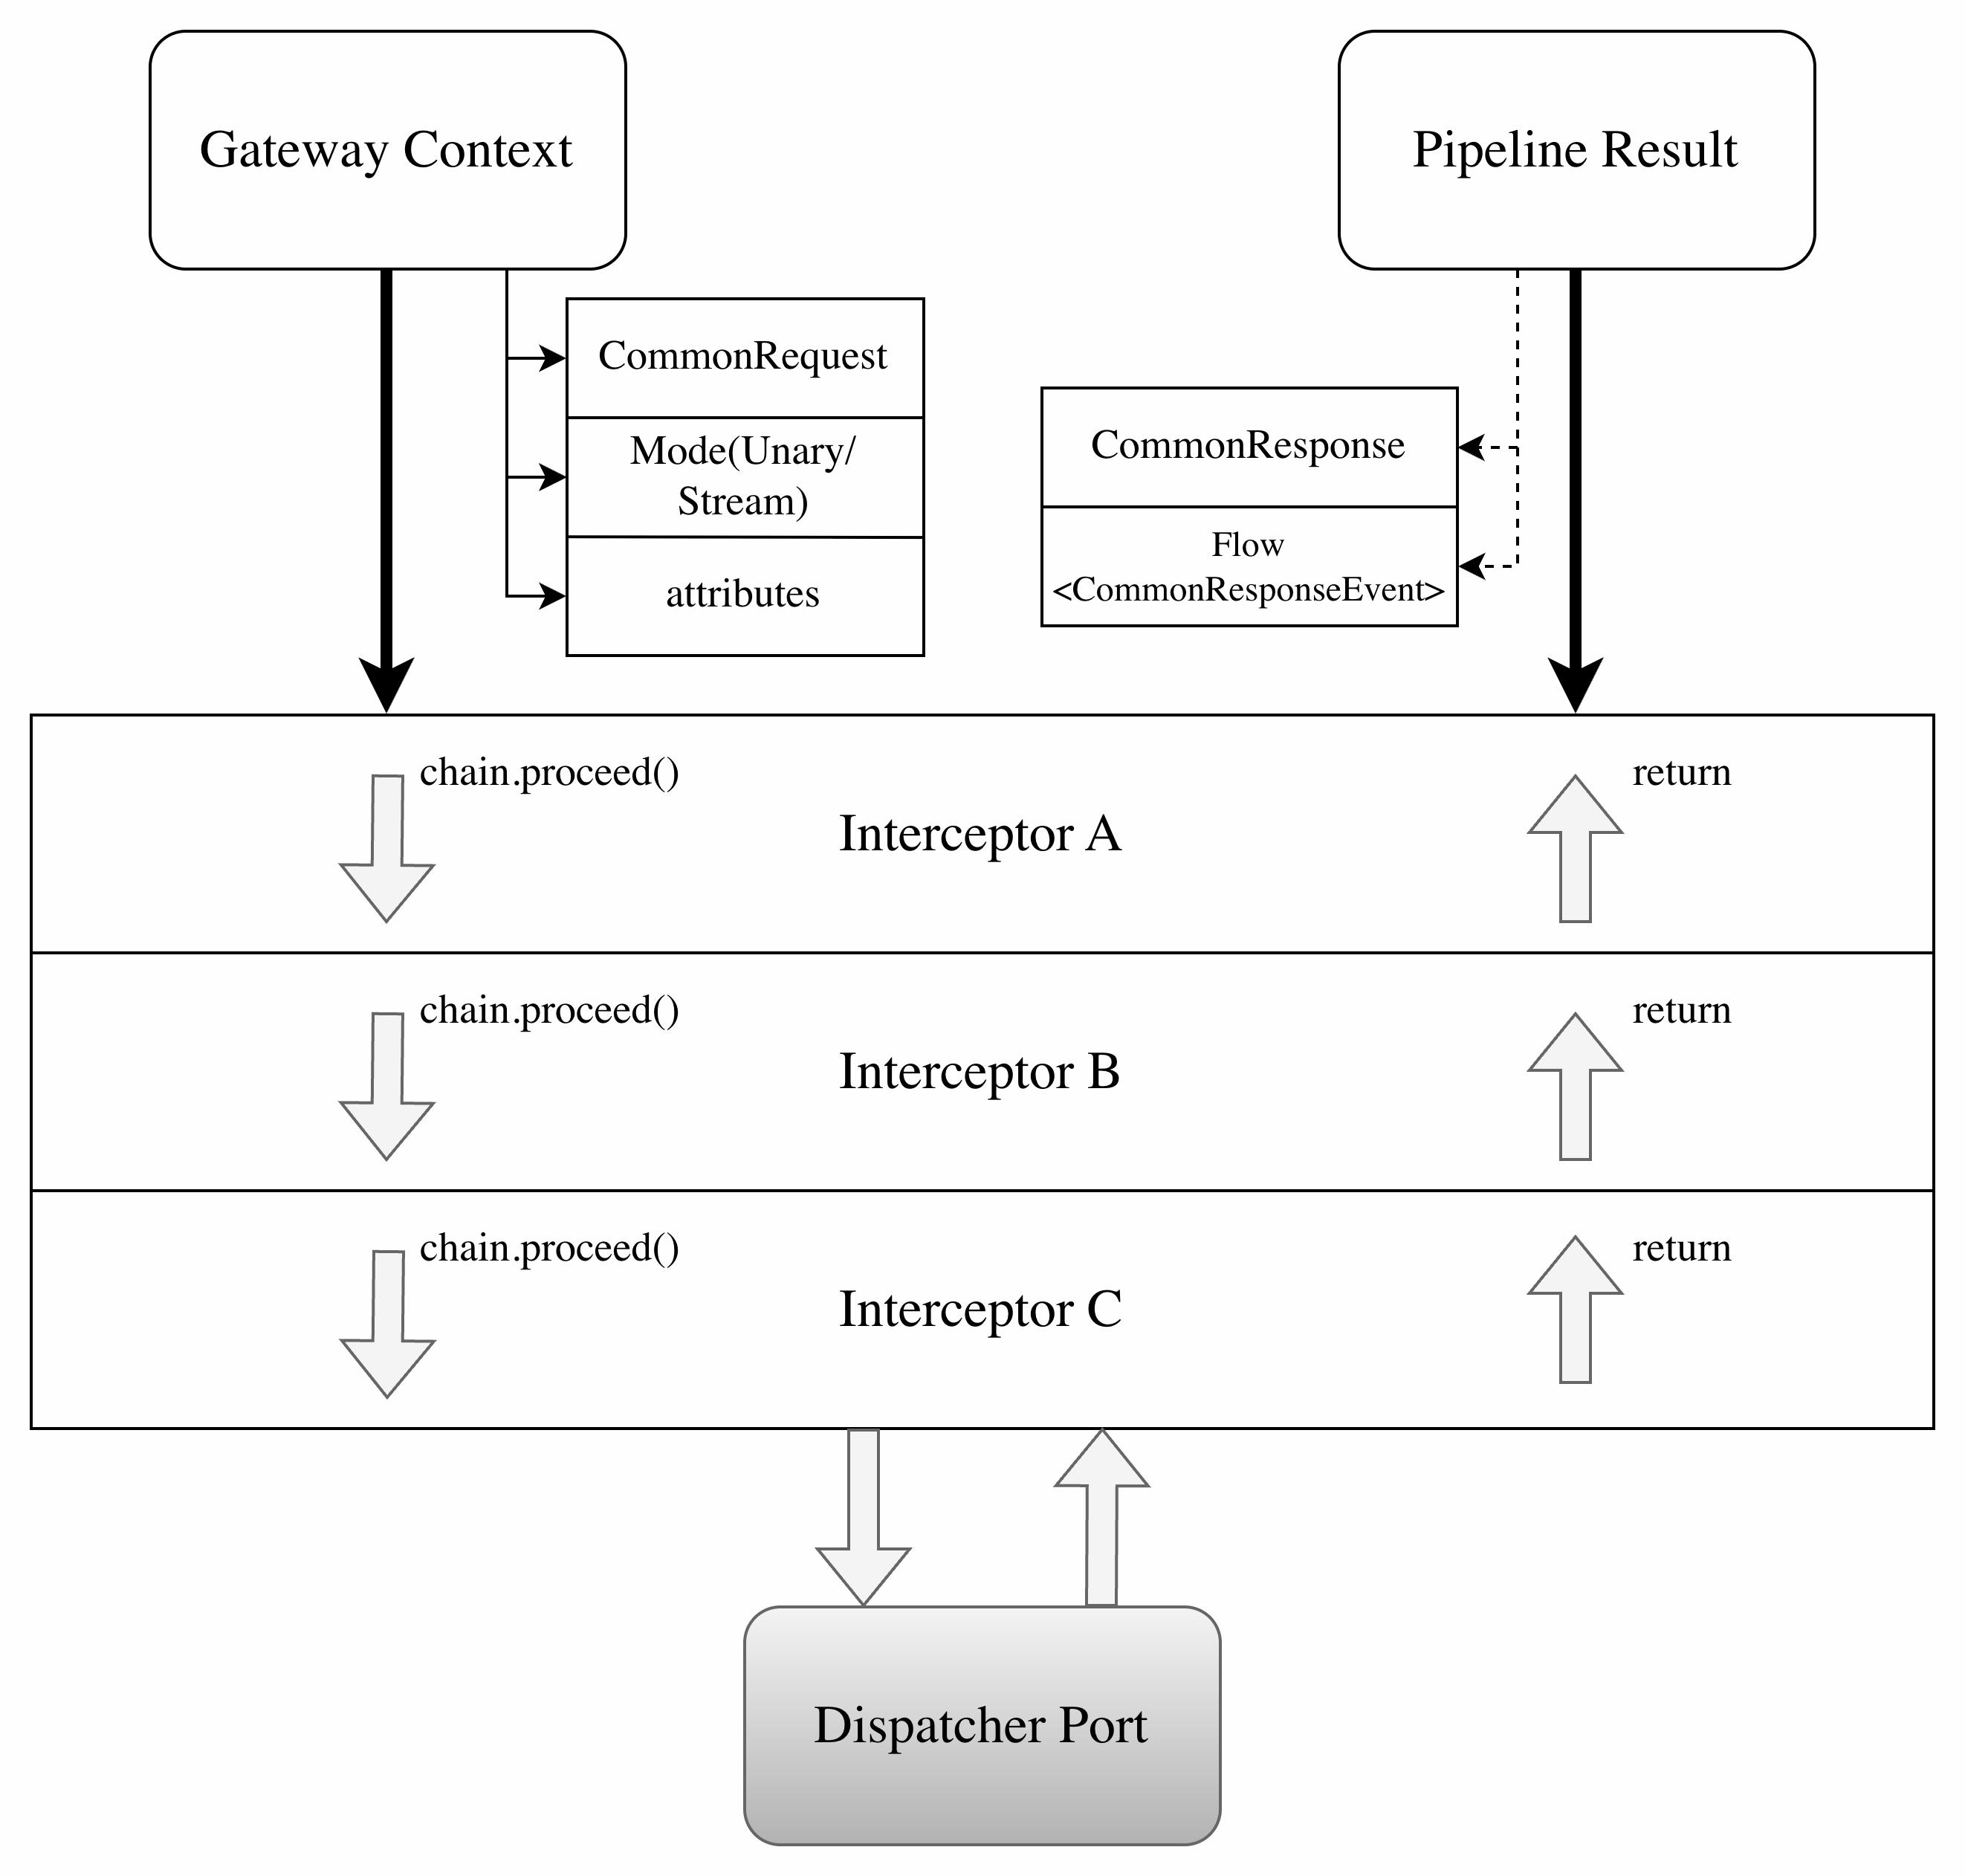
\includegraphics[width=0.9\textwidth]{../images/PipelineViewW.jpeg}
        \caption{Visão conceptual da \textit{pipeline} de \textit{interceptors}}
        \label{fig:pipeline}
    \end{figure}

    Esta forma mantém a arquitetura simples. O modelo é semelhante ao dos filtros de \textbf{Servlets} \cite{java_servlet_filterchain}: cada filtro recebe um contexto, decide se continua a cadeia e pode executar lógica antes e depois do próximo elemento. A diferença é que, no \textbf{OmniAI SDK}, o contexto não representa apenas um pedido \textbf{HTTP}; representa uma chamada de inferência já normalizada, incluindo fornecedor, modelo, modo de execução, atributos tipados e eventual fluxo de \textit{streaming}.

    A \textit{pipeline} é composta por \texttt{GatewayPipeline}, \texttt{GatewayPipelineChain}, \texttt{Interceptor} e \texttt{Gateway\allowbreak Context}. O \texttt{GatewayContext} transporta o pedido comum, atributos tipados e modo de execução, podendo representar chamadas síncronas ou \textit{streaming}. A cadeia executa os \textit{interceptors} por ordem e, no fim, invoca o \textit{dispatcher} terminal.

    Esta abordagem também prepara o escalamento horizontal. A \textit{pipeline} não exige estado global obrigatório; cada pedido transporta o seu contexto. Onde existe estado partilhável, como \textit{rate limiting} ou \textit{circuit breaker}, o \textbf{SDK} define \textit{stores} substituíveis. A implementação em memória é adequada para desenvolvimento e instância única, mas pode ser trocada por \textbf{Redis}, base de dados ou outro \textit{backend} coordenado em implantações distribuídas. Assim, várias instâncias da \textbf{OmniAI Gateway} podem partilhar contadores, estados de circuito e metadados operacionais sem alterar o contrato dos \textit{inbounds} nem a forma como os clientes chamam a \textbf{Gateway}.

    \section{Arquitetura Interna dos Interceptors}
    O módulo \texttt{interceptors} inclui implementações pré-construídas para preocupações operacionais e de segurança. Todos seguem o mesmo contrato: recebem um \texttt{GatewayContext}, consultam ou acrescentam atributos à \texttt{TypedMap}, decidem se chamam \texttt{chain.proceed(context)} e podem observar ou transformar o \texttt{PipelineResult}. Esta estrutura permite colocar lógica transversal antes e depois da inferência sem acoplar essa lógica aos \textit{adapters} de entrada, aos \textit{adapters} de saída ou ao \textit{dispatcher}.

    A ordem de execução é configurável. No \textit{target} \textbf{JVM}, o \textbf{SDK} suporta a anotação \texttt{Interceptor\allowbreak Priority}, usada para executar primeiro \textit{interceptors} com prioridade superior. No \textit{target} \textbf{JavaScript}, onde a reflexão sobre anotações é limitada, a ordem segue a sequência definida pela DSL. Assim, autenticação e autorização podem ocorrer no início da cadeia, enquanto métricas, \textit{tracing} e \textit{logging} podem envolver a execução completa.

    A motivação para estes \textit{interceptors} não foi apenas organizar código, mas tornar explícitas políticas que, numa \textbf{Gateway} de IA, afetam segurança, custo e disponibilidade. A Tabela~\ref{tab:interceptor-rationale} resume essa relação.

    \begin{table}[H]
        \centering
        \footnotesize
        \renewcommand{\arraystretch}{1.25}
        \begin{tabularx}{\textwidth}{|>{\raggedright\arraybackslash}p{3.2cm}|Y|Y|}
            \hline
            \textbf{Interceptor} & \textbf{Problema tratado} & \textbf{Motivo para estar na Gateway} \\
            \hline
            Telemetria & Falta de visibilidade sobre latência, erros, \textit{tokens} e fornecedores. & A \textbf{Gateway} observa todas as chamadas e consegue medir comportamento transversal sem alterar clientes ou \textit{adapters}. \\
            \hline
            Autenticação & Necessidade de validar quem apresenta o token antes de consumir modelos pagos. & A \textbf{Gateway} é o recurso protegido e deve validar \textit{tokens} antes de encaminhar tráfego para fornecedores. \\
            \hline
            Autorização & Um token válido não implica permissão para todos os modelos ou operações. & A decisão por cliente, ação, fornecedor e modelo deve ser centralizada antes da inferência. \\
            \hline
            Rate limiting & Risco de abuso, picos de carga e custos inesperados. & A \textbf{Gateway} é o ponto natural para aplicar quotas por cliente, plano, fornecedor ou modelo. \\
            \hline
            Circuit breaker & Dependências externas podem ficar lentas ou indisponíveis. & A \textbf{Gateway} evita insistir em fornecedores em falha e protege o restante sistema. \\
            \hline
            Fallback & Uma falha de fornecedor não deve, quando existe alternativa, falhar imediatamente a experiência do cliente. & A \textbf{Gateway} conhece os \textit{outbounds} disponíveis e pode tentar alternativas mantendo o contrato do cliente. \\
            \hline
        \end{tabularx}
        \caption{Justificação dos \textit{interceptors} fornecidos pelo \textbf{SDK}}
        \label{tab:interceptor-rationale}
    \end{table}

    \subsection{Interceptor de Telemetria e Observabilidade}
    O \texttt{MetricsInterceptor} recolhe dados operacionais essenciais num sistema que intermedeia chamadas a LLMs: latência, sucesso, erro, fornecedor, modelo, cliente e consumo de \textit{tokens}. Estes dados são importantes porque uma \textbf{Gateway} centraliza tráfego de vários clientes e fornecedores; sem telemetria, não é possível perceber custos, degradação, falhas por modelo ou impacto de políticas como \textit{fallback}.

    A implementação distingue chamadas unárias de \textit{streaming}. Em respostas progressivas, o \textit{interceptor} não bloqueia a execução; usa operadores de fluxo para observar eventos e emitir métricas no encerramento do \textit{stream}. Assim mede a duração total da interação, e não apenas o tempo até ao primeiro fragmento.

    A arquitetura segue inversão de dependência através da porta \texttt{MetricsPort}. O \textbf{OmniAI SDK} define primitivas de métricas comuns, como \texttt{counter}, \texttt{histogram} e \texttt{upDownCounter}, enquanto o \textit{adapter} concreto no \textit{target} \textbf{JVM} exporta para \textbf{OpenTelemetry}. O uso do \textbf{OpenTelemetry Protocol} (\textbf{OTLP}) foi escolhido porque o \textbf{OTLP} define a codificação, transporte e entrega de dados de telemetria entre fontes, coletores e \textit{backends} \cite{opentelemetry_otlp}. Esta escolha evita o acoplamento do \textbf{OmniAI SDK} a ferramentas específicas como \textbf{Prometheus}, \textbf{Grafana}, \textbf{Datadog} ou outro \textit{backend} específico: o \textbf{SDK} emite telemetria num formato aberto, o Collector recebe e processa esses dados, e a infraestrutura decide para onde exportar.

    Esta decisão é especialmente importante numa \textbf{Gateway} de IA. O mesmo \textbf{OmniAI SDK} pode ser usado por uma aplicação simples em desenvolvimento, por um POC local com \textbf{Prometheus}/\textbf{Grafana} ou por uma instalação futura com outro \textit{backend} de observabilidade. A \textbf{OpenTelemetry} apresenta-se precisamente como especificação aberta e agnóstica de fornecedor \cite{opentelemetry_what_is}; por isso, a instrumentação fica no \textbf{OmniAI SDK}, mas a escolha operacional do \textit{backend} permanece fora do domínio.

    \begin{figure}[H]
        \centering
        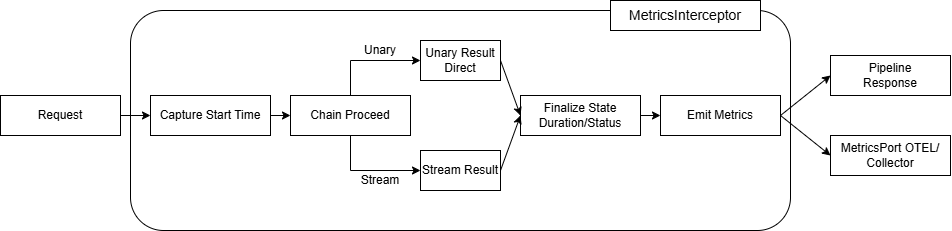
\includegraphics[width=0.9\textwidth]{../images/MetricsInterceptor.drawio.png}
        \caption{Fluxo interno de processamento e lógica de observabilidade para pedidos unários e \textit{streaming}}
        \label{fig:metrics-interceptor-arch}
    \end{figure}

    Para adicionar uma métrica, a aplicação usa a DSL do \texttt{gateway-client}. O utilizador pode ativar a latência padrão, acrescentar atributos globais e definir métricas próprias com uma função \texttt{value}, que extrai o valor a partir do contexto e do resultado, e uma função \texttt{tags}, que acrescenta dimensões de análise.

    \vspace{0.5em}
    \begin{lstlisting}[language=kotlin, caption={Configuração de telemetria e métricas personalizadas na DSL}]
        
metrics {
    metricsPort = telemetryRuntime.metricsPort
    tracer = telemetryRuntime.tracer

    attributes {
        include(ClientIpMetadataKey, alias = "client.ip")
        attribute("sdk.version") { _, _ -> "1.0.0" }
    }

    defaultLatency {
        enabled = true
        name = "gateway.inference.request.duration"
    }

    customMetrics {
        counter(
            name = "gateway.llm.tokens",
            description = "Total de tokens consumidos",
            unit = "{tokens}"
        ) {
            value { _, result ->
                (result as? PipelineResult.Unary)?.response?.usage?.totalTokens
            }
        }
    }
}
    \end{lstlisting}

    Este desenho separa três responsabilidades: a definição da métrica na DSL, a recolha no \textit{interceptor} e a exportação no \textit{adapter} de telemetria. Também facilita testes, porque \texttt{NoOpMetricsPort} pode ser usado quando a observabilidade está desligada.

    \begin{figure}[H]
        \centering
        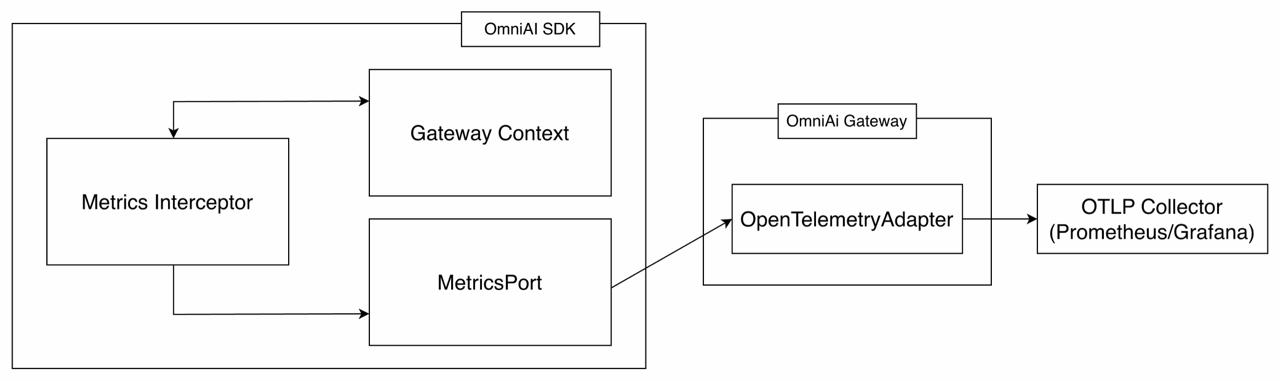
\includegraphics[width=0.9\textwidth]{../images/MetricsGateway}
        \caption{Observabilidade e métricas operacionais da \textbf{OmniAI Gateway}}
        \label{fig:metrics-gateway}
    \end{figure}

    \subsection{Interceptor de Autenticação}
    A autenticação é realizada pelo \texttt{AuthenticationInterceptor}. A \textbf{Gateway} atua como \textit{Resource Server}, recebe pedidos para recursos protegidos, extrai o \textit{access token} do cabeçalho \texttt{Authorization: Bearer <token>} e valida se esse token foi emitido por um servidor de autorização confiável \cite{rfc6749,rfc6750,oauth_resource_server}. Esta responsabilidade é essencial numa AI \textbf{Gateway}, porque a camada central passa a proteger acesso a modelos, custos, quotas e dados operacionais.

    A \textbf{Gateway} não deve atuar como \textit{Authorization Server}: não emite \textit{tokens}, não gere credenciais dos clientes e não substitui sistemas como \textbf{Logto} ou \textbf{Keycloak}. O seu papel é o de API protegida. Por isso, valida \textit{tokens} recebidos, confirma se foram emitidos para a audiência esperada e só depois permite que o pedido avance na \textit{pipeline} para os próximos \textit{interceptors}. Esta separação reduz responsabilidade de segurança dentro do \textbf{SDK} e permite integrar diferentes fornecedores de identidade sem alterar o contrato dos clientes.

    O fluxo inicia-se no \textit{adapter} \textbf{HTTP}, que propaga o token para o domínio através de metadados. O \textit{interceptor} classifica o token: se tiver três segmentos, é tratado como \textbf{JWT}; caso contrário, como token opaco. Esta distinção permite escolher entre validação local por assinatura e validação remota por introspeção.

    No modo \textit{OIDC Discovery} (RFC 8414), a \textbf{Gateway} obtém dinamicamente metadados do \textit{Authorization Server}, como \textit{issuer}, \texttt{jwks\_uri} e \textit{endpoint} de introspeção \cite{rfc8414}. Todo este fluxo encontra-se ilustrado na Figura 5.4. Para JWTs, valida o \texttt{kid}, obtém a chave pública no \textbf{JWKS}, verifica assinatura e confirma \textit{claims} como \texttt{exp}, \texttt{nbf}, \texttt{iss} e \texttt{aud} \cite{rfc7519,rfc7517,rfc7515}. Para \textit{tokens} opacos, usa introspeção \textbf{OAuth2} \cite{rfc7662}.

    \begin{figure}[H]
        \centering
        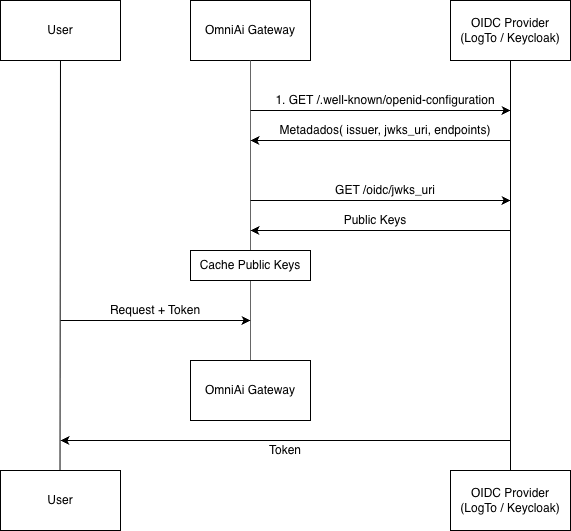
\includegraphics[width=0.9\textwidth]{../images/AutenticationFlow.png}
        \caption{Sequência \textbf{OIDC}: descoberta, \textbf{JWKS} e cache de chaves}
        \label{fig:oidc-sequence}
    \end{figure}

Para reduzir latência e chamadas repetidas ao servidor de autorização, a implementação inclui 
\texttt{InMemory\allowbreak KeyCache}, rotação de chaves em \textit{background} e um período de \textit{cooldown}. 
A rotação de chaves é realizada por uma \textit{coroutine} executada em segundo plano que, com um intervalo configurável, 
atualiza as chaves públicas do servidor de autorização. O \textit{cooldown} define um intervalo mínimo entre novas 
tentativas de obtenção de uma chave em falta, evitando consultas repetidas e mitigando alguns ataques ou abusos. A implementação de 
\texttt{InMemoryKeyCache}\allowbreak pode ser substituída por uma solução distribuída, como uma base de dados 
chave-valor, por exemplo o Redis. No caso de \textit{tokens} opacos, o \texttt{IntrospectionCache} usa 
\textit{positive caching} para \textit{tokens} ativos e \textit{negative caching} para \textit{tokens} inválidos. 
Os \textit{tokens} opacos são guardados em cache através de \textit{hash}, evitando manter credenciais em texto claro 
em memória.

O resultado é encapsulado em \texttt{Auth\allowbreak Validation\allowbreak Result} e guardado na \texttt{Typed\allowbreak Map} sob a chave \texttt{AUTH\_\allowbreak RESULT\_\allowbreak KEY}. Isto permite que autorização, métricas e \textit{logging} reutilizem a identidade já validada.

    \begin{figure}[H]
        \centering
        
\includegraphics[width=\textwidth]{../images/autenticacao}
        \caption{Fluxo interno do \textit{interceptor} de autenticação}
        \label{fig:auth-interceptor}
    \end{figure}

    A integração do processo de autenticação é declarada na montagem do \textit{SDK} usando a DSL correspondente:

\vspace{0.5em}
\begin{lstlisting}[language=kotlin, caption={DSL de configuração do \textit{interceptor} de autenticação com \textbf{OIDC} Discovery}]
security {
    authentication {
        discovery {
            discoveryUrl = "https://auth.example.com/.well-known/openid-configuration"
            expectedAudience = "https://gateway.example.com/api"
            clientId = "gateway-client" // Identificador publico da aplicacao cliente
            clientSecret = System.getenv("GATEWAY_CLIENT_SECRET") // Credencial para autenticacao junto do Provider
        }
    }
}
\end{lstlisting}

\subsection{Interceptor de Autorização}
A autorização é separada da autenticação porque responder a ``quem é o utilizador?'' não é o mesmo que responder a ``o que este utilizador pode fazer?''. A autenticação valida identidade; a autorização decide permissões sobre uma ação e um recurso. Esta separação é importante numa \textbf{Gateway} multi-cliente, onde um token válido pode não ter permissão para usar todos os modelos, fornecedores ou operações. A distinção entre autenticação e autorização é também a base dos modelos modernos de identidade, a primeira prova identidade, enquanto a segunda concede permissão sobre dados ou ações protegidas \cite{microsoft_authn_authz}.

No contexto do projeto, esta separação evita dois problemas. Primeiro, impede que a validação de token seja confundida com autorização total, um cliente autenticado pode estar limitado a um subconjunto de modelos, fornecedores ou quotas. Segundo, permite trocar a origem das decisões de autorização sem alterar a autenticação.

A decisão de autorização é realizada por um \textit{Policy Decision Point} (PDP), responsável por avaliar se uma determinada ação sobre um recurso deve ser permitida ou negada com base nas políticas definidas. Embora numa fase inicial a decisão possa operar de forma local e simples, o sistema está desenhado para que essa mesma decisão possa ser assegurada por um PDP externo, tal como o AuthZen \cite{ref_authZen} ou o OPA \cite{ref_OPA}. 

No \textbf{OmniAI SDK}, a autorização é centralizada no \texttt{Policy\allowbreak Enforcer\allowbreak Interceptor}. O componente atua como \textit{Policy Enforcement Point} (PEP), ou seja interceta o pedido, constrói um \texttt{Authorization\allowbreak Input} e delega a decisão ao PDP através da porta \texttt{Policy\allowbreak Decision\allowbreak Point\allowbreak Port}. A construção do \texttt{Authorization\allowbreak Input} é desacoplada através do \texttt{Authorization\allowbreak Input\allowbreak Provider}, uma porta que permite adaptar o contexto interno da \textbf{Gateway} ao formato esperado pelo motor de autorização. Desta forma, diferentes estratégias de extração de atributos podem ser utilizadas sem alterar o fluxo principal de autorização.

Podemos ver todo este fluxo na figura \ref{fig:authorization-architecture}.

\begin{figure}[H]
    \centering
    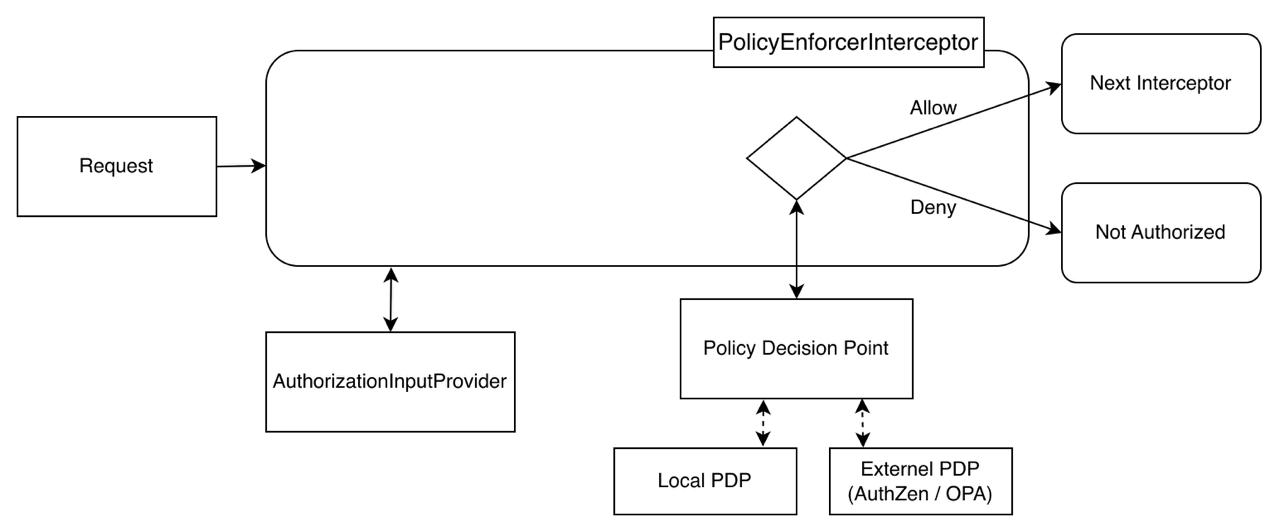
\includegraphics[width=0.9\textwidth]{../images/Authorization}
    \caption{Arquitetura do \textit{interceptor} de autorização: separação entre PEP e PDP}
    \label{fig:authorization-architecture}
\end{figure}

O \texttt{AuthorizationInput} segue o padrão \textbf{Subject-Action-Resource (SAR)}. O \textbf{Subject} representa o utilizador ou aplicação, incluindo identificador, roles e atributos vindos do token. A \textbf{Action} representa a operação, como \texttt{chat\_completion}. O \textbf{Resource} identifica o alvo, como fornecedor ou modelo. O \textbf{Context} acrescenta atributos extra caso seja necessarios.

A porta do PDP permite integrar motores diferentes, incluindo políticas internas, AuthZen \cite{ref_authZen}, OPA \cite{ref_OPA} ou outro serviço externo. Se a decisão for \textit{Deny}, a \textit{pipeline} é interrompida antes de qualquer chamada ao fornecedor \cite{authorization_pips}.

\vspace{0.5em}

\begin{lstlisting}[language=kotlin, caption={Porta para construção do contexto de autorização}]

fun interface AuthorizationInputProvider {
    fun getAuthorizationInput(context: GatewayContext): AuthorizationInput
}

data class AuthorizationInput(
    val subject: Subject,
    val action: Action,
    val resource: Resource,
    val context: Map<String, Any> = emptyMap(),
)
\end{lstlisting}

A configuração de autorização usando DSL:

\vspace{0.5em}
\begin{lstlisting}[language=kotlin, caption={DSL de configuração do \textit{interceptor} de autorização}]

security {
    authorization {
        pdp = customPolicyDecisionPoint
        inputProvider = DefaultAuthorizationInputProvider
    }
}
\end{lstlisting}


    \subsection{Interceptor de \textit{Rate Limiting} }
    O \texttt{RateLimitInterceptor} aplica limites de utilização antes da chamada ao fornecedor. Numa AI \textbf{Gateway}, este mecanismo tem dois objetivos principais: proteger o sistema contra abuso ou tráfego excessivo e controlar custos associados a chamadas de inferência. A limitação de taxa é uma estratégia comum para impor um teto de ações repetidas num intervalo temporal, reduzindo abuso de APIs, força bruta e carga excessiva \cite{cloudflare_rate_limiting}.

    A importância deste \textit{interceptor} é maior do que numa API tradicional, porque cada pedido pode representar custo financeiro direto, consumo de quotas externas e ocupação prolongada de ligações em \textit{streaming}. Sem \textit{rate limiting}, um cliente mal configurado, uma automação em ciclo ou um utilizador abusivo pode saturar a \textbf{Gateway}, esgotar quotas nos fornecedores e degradar o serviço para clientes legítimos. O \textit{interceptor} permite aplicar justiça operacional: cada cliente, plano, modelo ou fornecedor pode ter limites próprios.

    A lógica é orientada por políticas. Cada \texttt{RateLimitPolicy} extrai dados do \texttt{GatewayContext} e devolve \texttt{RateLimitTarget}. Um \textit{target} contém uma chave, como cliente/modelo/plano, e uma \texttt{RateLimitDefinition}, composta por limite, tipo e janela temporal. Isto permite políticas diferentes por cliente, plano, modelo ou fornecedor.

    O store atual em memória usa buckets protegidos por \texttt{Mutex}. Quando um pedido chega, o \textit{interceptor} tenta consumir uma unidade em todos os buckets aplicáveis. Se todos permitirem consumo, a cadeia continua. Se algum limite estiver esgotado, devolve \texttt{TooManyRequestsError} com \texttt{retryAfter}. Esta resposta permite que clientes bem comportados reduzam ritmo em vez de insistirem. Para desenvolvimento e instância única, este modelo é suficiente; em escalamento horizontal, o contrato \texttt{RateLimitStore} permite substituir a implementação por \textbf{Redis} ou outro \textit{backend} partilhado. Essa substituição é necessária quando várias instâncias da \textbf{Gateway} devem partilhar a mesma visão de quota.

    A configuração deste mecanismo recorre ao seguinte bloco:

    \vspace{0.5em}
    \begin{lstlisting}[language=kotlin, caption={DSL de configuração do \textit{interceptor} de \textit{rate limiting}}]

interceptors {
    rateLimiting {
        store = InMemoryRateLimitStore()
        addPolicy(rateLimitPolicy)
    }
}
    \end{lstlisting}

    \subsection{Interceptor de \textit{Circuit Breaker}}
    O \texttt{CircuitBreakerInterceptor} protege a \textbf{Gateway} contra chamadas repetidas a um \textit{outbound} em falha. O padrão de \textit{circuit breaker} é usado para lidar com falhas em serviços remotos, evitando insistir numa dependência que está indisponível e dando tempo para recuperação \cite{microsoft_circuit_breaker,itau_circuit_breaker,treinaweb_circuit_breaker}. Numa \textbf{Gateway} de IA, esta proteção é especialmente útil porque fornecedores externos podem falhar por indisponibilidade, \textit{timeouts}, quotas ou erros 5xx.

    A alternativa simples seria repetir pedidos até obter sucesso. Essa abordagem é perigosa quando o fornecedor está realmente indisponível: as tentativas acumulam latência, ocupam \textit{threads} ou corrotinas, aumentam custos e podem agravar a falha no serviço externo. O \textit{circuit breaker} foi criado para evitar esse comportamento. Quando a falha ultrapassa um limiar, o circuito abre e a \textbf{Gateway} passa a falhar rapidamente aquele destino, libertando recursos e permitindo que mecanismos como \textit{fallback} escolham outro \textit{outbound}.

    Para cada combinação de fornecedor/modelo, o \textit{interceptor} identifica o \texttt{outbound.key} e consulta o \texttt{CircuitBreakerStore}. Se o circuito estiver \texttt{OPEN}, o pedido falha rapidamente com \texttt{ApiDownError} e o \textit{outbound} é acrescentado ao conjunto de \textit{outbounds} negados no contexto. Esta falha rápida reduz latência, evita consumo de recursos e dá ao \textit{fallback} informação para não tentar novamente o mesmo destino.

    Quando a chamada prossegue, o \textit{interceptor} observa o resultado. Erros incrementam o contador de falhas; ao atingir \texttt{failureThreshold}, o circuito passa para \texttt{OPEN}. Após um período de recuperação, o estado \texttt{HALF\_OPEN} permite testar um número limitado de pedidos antes de voltar ao estado \texttt{CLOSED}, evitando inundar um fornecedor que ainda está a recuperar \cite{microsoft_circuit_breaker}. A configuração inclui \texttt{failureThreshold}, \texttt{resetTimeoutMs} e \texttt{halfOpenTestRequests}. A implementação atual cobre a abertura e fecho básico do circuito; a evolução temporal mais completa do estado \texttt{HALF\_OPEN} é uma melhoria natural.

    \vspace{0.5em}
    \begin{lstlisting}[language=kotlin, caption={DSL de configuração do \textit{interceptor} de \textit{circuit breaker}}]

interceptors {
    circuitBreaker {
        store = InMemoryCircuitBreakerStore()
        config = CircuitBreakerConfig(
            failureThreshold = 5,
            resetTimeoutMs = 10000L,
            halfOpenTestRequests = 2
        )
    }
}
    \end{lstlisting}

    \subsection{Interceptor de \textit{Fallback}}
    O \texttt{FallbackInterceptor} permite tentar alternativas quando a chamada principal falha. Em sistemas de IA, \textit{fallback} ao nível de modelo ou fornecedor é relevante porque falhas nas APIs de inferência fornecidas pelas LLMs são um cenário frequente em produção: \textit{rate limits}, indisponibilidade, quotas, \textit{timeouts} ou modelos descontinuados podem impedir a resposta do fornecedor principal \cite{ai_fallback_tombas,portkey_fallback}. Um \textit{gateway} é o ponto certo para esta política, porque conhece os \textit{outbounds} configurados e consegue trocar de destino sem exigir alterações no cliente.

    A decisão de colocar \textit{fallback} na \textbf{Gateway}, e não nos clientes, reduz duplicação e melhora controlo operacional. Se cada aplicação cliente implementasse a sua própria lógica de \textit{fallback}, seria necessário repetir regras de prioridade, tratamento de erros, mapeamento de contratos e métricas em vários pontos. Ao centralizar a política, o \textbf{SDK} consegue manter o mesmo contrato de entrada e decidir internamente que fornecedor ou modelo alternativo deve ser tentado. Isto é particularmente útil quando o cliente usa um contrato compatível com \textbf{Anthropic} ou \textbf{OpenAI}, mas a \textbf{Gateway} pode executar a chamada noutro \textit{provider} configurado.

    A implementação atual usa a lista de \textit{outbounds} disponíveis. Primeiro tenta o \textit{outbound} correspondente ao fornecedor e modelo pedidos; se falhar, acrescenta esse \textit{outbound} ao conjunto de negados e tenta alternativas. Para cada tentativa, cria um novo \texttt{GatewayContext} com os mesmos atributos, mas com \texttt{provider} e \texttt{model} atualizados para o \textit{outbound} alternativo.

    A integração com o \textit{circuit breaker} é feita através do conjunto partilhado de \textit{outbounds} negados. Assim, se um circuito estiver aberto, o \textit{fallback} evita esse destino e tenta outro modelo ou fornecedor. Este desenho permite construir políticas de resiliência como ``tentar \textbf{Gemini}, depois \textbf{OpenAI}-compatible via \textbf{Groq}, depois \textbf{Anthropic}'', mantendo a lógica de tentativa fora dos \textit{adapters}. Também permite distinguir degradação controlada de erro total: a resposta pode chegar por um modelo alternativo, enquanto métricas e \textit{tracing} registam que ocorreu \textit{fallback}.

    A evolução futura poderá acrescentar prioridades configuráveis, condições por código de erro, orçamentos de tentativa e métricas específicas de \textit{fallback}. Estas regras são importantes porque nem todo erro justifica \textit{fallback}: erros de autenticação ou autorização devem falhar imediatamente, enquanto \textit{timeouts}, 429 e 5xx podem justificar uma alternativa.

    A sua ativação é extremamente simples, não requerendo configuração intrincada:

    \vspace{0.5em}
    \begin{lstlisting}[language=kotlin, caption={DSL de configuração do \textit{interceptor} de \textit{fallback}}]
interceptors {
    fallback()
}
    \end{lstlisting}

    \subsection{Interceptor de \textit{Logging} e \textit{Tracing}}
    O \texttt{RequestLoggingInterceptor} regista fornecedor, modelo, sucesso, erro e conclusão de streams através da abstração \texttt{GatewayLogger}. No \textit{target} \textbf{JVM} pode ser ligado a \textbf{SLF4J}; no \textit{target} \textbf{JavaScript} pode usar consola ou outra integração. O objetivo é garantir visibilidade mínima mesmo quando a telemetria completa não está ativa.

    O \textit{logging} foi mantido separado das métricas porque responde a perguntas diferentes. Métricas mostram tendências agregadas, como latência média ou número de erros; \textit{logs} ajudam a explicar um pedido concreto. Numa \textbf{Gateway} de IA, esta distinção também tem impacto de privacidade: o objetivo é registar metadados operacionais, e não despejar \textit{prompts}, respostas completas ou \textit{tokens} sensíveis nos \textit{logs}.

    O \texttt{TracingInterceptor} envolve o pedido num \textit{span} chamado \texttt{gateway.request.process}. Quando combinado com \textbf{OpenTelemetry}, este \textit{span} permite correlacionar latência, erros, chamadas externas e métricas agregadas. Em cenários de \textit{fallback} ou \textit{circuit breaker}, \textit{tracing} é particularmente útil porque permite observar o percurso real do pedido e distinguir falhas do fornecedor, decisões da \textbf{Gateway} e erros de cliente. Também permite perceber se uma resposta lenta resulta do fornecedor principal, de uma tentativa alternativa, de validação de token ou de uma política interna.

    A instalação processa-se em dois blocos da DSL, um explícito e outro decorrente da configuração de métricas:

    \vspace{0.5em}
    \begin{lstlisting}[language=kotlin, caption={Instalação dos \textit{interceptors} de \textit{logging} e \textit{tracing}}]
interceptors {
    // Instalacao manual do Logging Interceptor
    use(RequestLoggingInterceptor(logger))
    
    // O TracingInterceptor e instalado automaticamente ao fornecer o tracer as metricas
    metrics {
        tracer = telemetryRuntime.tracer
    }
}
    \end{lstlisting}



   \section{Distribuição Multiplataforma}

Um dos objetivos do \textbf{OmniAI SDK} é permitir que a lógica central da abstração de modelos seja reutilizada em diferentes ambientes de execução. O ecossistema \textbf{Kotlin Multiplatform} permite separar o código agnóstico das implementações específicas: o domínio, os contratos, as portas, os adaptadores principais, a DSL e parte dos \textit{interceptors} residem em \textit{source sets} comuns; por sua vez, os detalhes de infraestrutura como o cliente \textbf{HTTP}, a reflexão de prioridades, a integração com o servidor \textbf{Ktor} e as pontes de plataforma ficam isolados em \textit{source sets} específicos.

No \textit{target} \textbf{JVM}, o \textbf{OmniAI SDK} pode ser consumido nativamente por aplicações \textbf{Kotlin} ou Java. Este é o ambiente mais maduro no estado atual do projeto, sendo a fundação sobre a qual a nossa instância de demonstração (POC) do \textbf{OmniAI Gateway} foi construída. A implementação \textbf{JVM} inclui o cliente \textbf{HTTP} \textbf{Ktor}, a integração nativa com o servidor \textbf{Ktor}, a autenticação baseada em descoberta \textbf{OIDC}, a telemetria e a execução real dos \textit{outbounds}. A futura distribuição via \textbf{Maven} permitirá que qualquer aplicação adicione o \textbf{SDK} como uma dependência versionada clássica, eliminando a necessidade de recorrer a \textit{composite builds}.

Relativamente ao \textit{target} \textbf{JavaScript}/\textbf{Node.js}, o projeto prepara a disponibilização de uma API consumível a partir do ecossistema \textbf{TypeScript}. A utilização da anotação \texttt{@JsExport} atua como uma fachada que encapsula a configuração em tipos exportáveis, garantindo que as estruturas internas do \textbf{Kotlin} não transbordam de forma inadequada para a fronteira JS. Esta camada estabelece as fundações para o consumo via \textbf{NPM}, embora ainda não apresente paridade total de funcionalidades com o ambiente \textbf{JVM}.

A principal premissa desta arquitetura multiplataforma é a de que nem todos os componentes devem ser partilhados. Enquanto o domínio e os contratos devem permanecer estritamente comuns e agnósticos, as camadas de transporte \textbf{HTTP}, servidor, observabilidade e segurança podem e devem ter implementações otimizadas para cada plataforma. Esta fronteira arquitetural evita a duplicação de código sem forçar uma abstração demasiado rígida ou ineficiente. A linha de evolução natural passa por consolidar a API pública do \textbf{OmniAI SDK}, estabilizar o versionamento semântico, automatizar a publicação \textbf{Maven}/\textbf{NPM} através de \textit{Continuous Delivery} (CD) e documentar exemplos mínimos de consumo para a \textbf{JVM} e \textbf{Node.js}.
